\chapter{Experimentální metody}

\section{Metoda téměř zkřížených polarizátorů}
\subsection{Teorie}
Toto experimentální uspořádání umožňuje rychlé určení Kerrovy rotace a elipsity pro celé spektrum. V našem případě používáme CCD spektometr v kombinaci se širokospektrálním zrojem, který se skládá z halogenové a deuteriové výbojky. To umožňuje proměření celého spektra najednou. Schéma celého experimentu je zobrazeno na obrázku (\ref{Schéma rotující polarizátor}). Ze zdroje je světlo vedeno optickým vláknem do aparatury. Svazek je nejprve kolimován spojnou čočkou. Následně prochází polarizátorem, který je otočen o úhel $\alpha$ od svislé osy a fázovou destičkou s fázovým posuvem $\delta$. Po odrazu na vzorku prochází světlo analyzátorem, který je natočený o úhel $\pi/2$ od svilé osy. Výstupní světlo je zachyceno sběrnou čočkou do optického vlákna, které vede do spektrometru. Za pomoci Jonesova formalizmu můžeme spočítat Jonesův vektor světla dopadajícího na detektor.
\begin{eqnarray}
J=r\begin{bmatrix}0&0\\0&1\end{bmatrix}\begin{bmatrix}1&-\Theta_K\\-\Theta_K&-1\end{bmatrix}\begin{bmatrix}e^{i\frac{\delta}{2}}&0\\0&e^{-i\frac{\delta}{2}}\end{bmatrix}\begin{bmatrix}\cos\alpha\\\sin\alpha\end{bmatrix}\\
=r\begin{bmatrix}0\\-\Theta_Ke^{i\frac{\delta}{2}}\cos\alpha+e^{-i\frac{\delta}{2}}\sin\alpha\end{bmatrix},
\end{eqnarray}
kde $r$ značí reflexní koeficient vzorku. Pro intenzitu světla u sběrné čočky pak máme
\begin{eqnarray}
I\approx\frac{1}{2}JJ^*=\frac{R}{2}(\sin^2\alpha+|\Theta_K|^2\cos^2\alpha+\sin(2\alpha)\mbox{Re}(\Theta_Ke^{i\delta}))
\label{I1}
\end{eqnarray}
Nyní můžeme použít přiblížení pro malé elipsometrické úhly, pro které platí
\begin{eqnarray}
\Theta_K\approx\theta_K-i\epsilon_K
\end{eqnarray}
Výraz (\ref{I1}) se pak redukuje na
\begin{eqnarray}
I\approx\frac{R}{2}(\sin^2\alpha+(\theta_K\cos\delta+\epsilon_K\sin\delta)\sin(2\alpha))
\label{I2}
\end{eqnarray}
V  případě, že $\delta=0$, tedy odebereme fázovou destičku, nám zcela vymizí elipticita. Fitováním naměřených dat v závislost na úhlu natočení polarizátoru $\alpha$ pak můžeme získat přímo rotaci. Pro určení elipticity následně naměříme i hodnoty s fázovou destičkou. V ideáním případě bychom použili půlvlnnou destičku, ale vzhledem k tomu, že její fáze je funkcí vlnové délky, musíme počítat s tím, že fitovaný parametr při druhém měření odpovídá celému výrazu $K=(\theta_K\cos\delta+\epsilon_K\sin\delta)$. Rotaci známe z prvního měření a $\delta$ určíme z kalibrační funkce destičky. Elipticita se nakonec rovná
\begin{eqnarray}
\epsilon_K=(K-\theta_K\cos\delta)/\sin\delta
\end{eqnarray}

Tato závislost předpokádá přesné určení vzájemné polohy polarizátorů. Tu však v praxi neznáme a proto využíváme toho, že platí $\theta_K(M)=-\theta_K(-M)$. kde $M$ značí magnetizaci. Měříme tedy závislosti pro dva opačné proudy procházející magnetem a výsledné nafitované konstanty od sebe odečteme a vydělíme dvěmi.

\subsection{Použitá zařízení}
Fotografii celé aparatury můžete vidět na obrázku (\ref{TPE photo}).

\begin{figure}
\begin{center}
\includegraphics[width=5in]{img/TPEPhoto.eps}
\caption{Fotografie aparatury pro metodu skřížených polarizátorů}
\label{TPE photo}
\end{center}
\end{figure}

Jako zdroj světla používáme lampu typ XXX od Ocean Optics. Obě najedou pokrývají spektrální rozsah od 250 nm do 1000 nm. Náš zdroj umožňuje použití obou trubic zároveň, avšak heliová trubice vytváří světlo o přibližně pětkrát větší intenzitě. Z toho důvodu je v oblasti malých vlnových délek znatelně vyšší šum. Dostatečná doba integrace signálu však tento šum téměř zcela vyruší.

Polarizátory z CaF a křemene typu Rochon jsou umístěny do držáků s krokovými motorky.  Ty umožňují nastavení úhlu s přesností až $10^{-3}$ stupně. Jejich ovládání je zprostředkováno kontrolní jednotkou DC 500 od společnosti Owis. Ta umožňuje jejich manuální ovládání i kontrolu přes rozhraní GPIB.

V našem uspořádání vytváří magnet polární magnetické pole. Aby nedocházelo ke zahřívání vzorku, je celý magnet chlazený studenou vodou. Při proudu 2 A vytváří magnet pole okolo 0.4 T, které bylo dostatečné k nasycení měřených vzorků. %TODO Hysterzní smyška

K analýze světla používáme CCD spektrometr USB2000+ od Ocean Optics. Jeho schéma naleznete na obrázku (\ref{USB2000+ schema}). Rozsah spektrometru je přibližně od 200 do 900 nm s rozlišovací schopností (doplň číslo). Komunikace se spektrometrem je zprostředkována přes rozhraní USB protokolem VISA. 

\subsection{Průběh měření}
Samotné měření se dá rozdělit do dvou částí. První je nastavení aparatury a druhá samotné měření. Toto rozdělení respektuje i ovládací program.
\subsubsection{Nastavení aparatury}
Po upevnění vzorku je nejprve třeba navést světelný svazek do vlákna spektrometru. Ač je na jeho začátku sběrná čočka, je třeba velmi jemného nastavení za pomoci aretačních šroubů, protože natočení této čočky má velký vliv na měřenou intenzitu.

Následně je potřeba nastavit první polarizátor tak abychom získali p-polarizované světlo. Proto za něj umístíme sklíčko tak jak je ukázáno na obrázku (\ref{TPE install}). Úhel odrazu od sklíčka odpovídá Brewsterově úhlu, z čehož vyplývá, že při nastavení polarizátoru na p-polarizaci detekujeme minimální intenzitu světla. To platí nezávisle na vlnové délce, proto je nejvhodnější vyhodnocovat pouze neiintenzivnější část spektra. Minimum nalezneme tak, že proskenujeme různé úhly natočení polarizátoru a následně zhustšujeme měření v oblasti minima, dokud nedosáhneme požadované přesnosti.

Druhý polarizátor je nutné pouze zkřížit, aby měřené závislosti byli co nejsymetričtější, což usnadňuje fitování. Toho docílíme podobně jako u prvního, protože se opět jedná o hledání minima signálu při nulovém magnetickém poli.

Aby nebylo nutné nastavovat aparaturu před každým měřením, jsou natočení polarizátoru uchovávány v externím souboru a při spuštění programu se použijí, pokud nastavování neproběhne. Díky tomu je kalibrace nutná pouze v případě zásahu do aparatury. 


\subsection{Měření}
Na začátku měření zadáme rozsah úhlu, které budeme měřit, krok, četnost měření spekter pro jednotlivé úhly a proud pro magnet. Tyto údaje mají velký vliv na úroveň šumu spektra a na dobu měření. Spektra při různých hodnotách jsou znázorněna na obrázcích (\ref{TPE1}) až (\ref{TPE3}) spektra při změnách těchto parametrů. Při našem nastavení stačí pro hrubý odhad spektra okolo 40 měření při četnosti 100. Takové měření trvá několik málo minut. Pokud však chceme minimální šum, měříme v rozahu od -40 do 40 stupňů s krokem 0.5 stupně a četnosti 500. Toto měření již trvá okolo 40 minut, ale jak je vidět na spektrech, výsledky jsou výrazně hladší.

Pro fitování předepsané závislosti (\ref{I2}) používáme Krameriovu metodu. Vzhledek k posunu nulové intenzity na detektoru je konečná fitovaná závislost
\begin{eqnarray}
I(\alpha)=a_1+a_2\sin^2(\alpha)+a_3\sin(2\alpha)
\end{eqnarray}
kde $a_1$ odpovídá zmíněnému posunu, $a_2$ je úměrné reflektivitě vzroku, ale vzhledem ke ztrátám na optických prvcích a v optickém vlákně nemá přílišný význam a z $a_3$ dopočteme za pomoci vztahu $\frac{a_3}{a_2}=(\theta_K\cos\delta+\epsilon_K\sin\delta)$ příslušný elisometrický koeficient, jak už bylo zmíněno výše. Ukázku naměřený závislosti pro $\lambda=$ !!DOPLN!! nm s nafitovanými křivkami naleznete na obrázku (\ref{TPE0}).

\begin{figure}
\input{grafy/TPE0}
\caption{Naměřená závislost intenzity na úhlu natočení polarizátoru pro $\lambda =$}
\label{TPE0}
\end{figure}

\begin{figure}
\input{grafy/TPE1}
\caption{Naměřené spektrum v pro různé množství měřených úhlů.}
\label{TPE1}
\end{figure}

\begin{figure}
\input{grafy/TPE2}
\caption{Naměřené spektrum v pro různé integrační doby spektra.}
\label{TPE2}
\end{figure}

\begin{figure}
% GNUPLOT: LaTeX picture with Postscript
\begingroup
  \makeatletter
  \providecommand\color[2][]{%
    \GenericError{(gnuplot) \space\space\space\@spaces}{%
      Package color not loaded in conjunction with
      terminal option `colourtext'%
    }{See the gnuplot documentation for explanation.%
    }{Either use 'blacktext' in gnuplot or load the package
      color.sty in LaTeX.}%
    \renewcommand\color[2][]{}%
  }%
  \providecommand\includegraphics[2][]{%
    \GenericError{(gnuplot) \space\space\space\@spaces}{%
      Package graphicx or graphics not loaded%
    }{See the gnuplot documentation for explanation.%
    }{The gnuplot epslatex terminal needs graphicx.sty or graphics.sty.}%
    \renewcommand\includegraphics[2][]{}%
  }%
  \providecommand\rotatebox[2]{#2}%
  \@ifundefined{ifGPcolor}{%
    \newif\ifGPcolor
    \GPcolorfalse
  }{}%
  \@ifundefined{ifGPblacktext}{%
    \newif\ifGPblacktext
    \GPblacktexttrue
  }{}%
  % define a \g@addto@macro without @ in the name:
  \let\gplgaddtomacro\g@addto@macro
  % define empty templates for all commands taking text:
  \gdef\gplbacktext{}%
  \gdef\gplfronttext{}%
  \makeatother
  \ifGPblacktext
    % no textcolor at all
    \def\colorrgb#1{}%
    \def\colorgray#1{}%
  \else
    % gray or color?
    \ifGPcolor
      \def\colorrgb#1{\color[rgb]{#1}}%
      \def\colorgray#1{\color[gray]{#1}}%
      \expandafter\def\csname LTw\endcsname{\color{white}}%
      \expandafter\def\csname LTb\endcsname{\color{black}}%
      \expandafter\def\csname LTa\endcsname{\color{black}}%
      \expandafter\def\csname LT0\endcsname{\color[rgb]{1,0,0}}%
      \expandafter\def\csname LT1\endcsname{\color[rgb]{0,1,0}}%
      \expandafter\def\csname LT2\endcsname{\color[rgb]{0,0,1}}%
      \expandafter\def\csname LT3\endcsname{\color[rgb]{1,0,1}}%
      \expandafter\def\csname LT4\endcsname{\color[rgb]{0,1,1}}%
      \expandafter\def\csname LT5\endcsname{\color[rgb]{1,1,0}}%
      \expandafter\def\csname LT6\endcsname{\color[rgb]{0,0,0}}%
      \expandafter\def\csname LT7\endcsname{\color[rgb]{1,0.3,0}}%
      \expandafter\def\csname LT8\endcsname{\color[rgb]{0.5,0.5,0.5}}%
    \else
      % gray
      \def\colorrgb#1{\color{black}}%
      \def\colorgray#1{\color[gray]{#1}}%
      \expandafter\def\csname LTw\endcsname{\color{white}}%
      \expandafter\def\csname LTb\endcsname{\color{black}}%
      \expandafter\def\csname LTa\endcsname{\color{black}}%
      \expandafter\def\csname LT0\endcsname{\color{black}}%
      \expandafter\def\csname LT1\endcsname{\color{black}}%
      \expandafter\def\csname LT2\endcsname{\color{black}}%
      \expandafter\def\csname LT3\endcsname{\color{black}}%
      \expandafter\def\csname LT4\endcsname{\color{black}}%
      \expandafter\def\csname LT5\endcsname{\color{black}}%
      \expandafter\def\csname LT6\endcsname{\color{black}}%
      \expandafter\def\csname LT7\endcsname{\color{black}}%
      \expandafter\def\csname LT8\endcsname{\color{black}}%
    \fi
  \fi
  \setlength{\unitlength}{0.0500bp}%
  \begin{picture}(7200.00,5040.00)%
    \gplgaddtomacro\gplbacktext{%
      \csname LTb\endcsname%
      \put(1342,704){\makebox(0,0)[r]{\strut{}-0.02}}%
      \put(1342,1213){\makebox(0,0)[r]{\strut{}-0.015}}%
      \put(1342,1722){\makebox(0,0)[r]{\strut{}-0.01}}%
      \put(1342,2231){\makebox(0,0)[r]{\strut{}-0.005}}%
      \put(1342,2740){\makebox(0,0)[r]{\strut{} 0}}%
      \put(1342,3248){\makebox(0,0)[r]{\strut{} 0.005}}%
      \put(1342,3757){\makebox(0,0)[r]{\strut{} 0.01}}%
      \put(1342,4266){\makebox(0,0)[r]{\strut{} 0.015}}%
      \put(1342,4775){\makebox(0,0)[r]{\strut{} 0.02}}%
      \put(1731,484){\makebox(0,0){\strut{} 300}}%
      \put(2587,484){\makebox(0,0){\strut{} 400}}%
      \put(3444,484){\makebox(0,0){\strut{} 500}}%
      \put(4300,484){\makebox(0,0){\strut{} 600}}%
      \put(5156,484){\makebox(0,0){\strut{} 700}}%
      \put(6013,484){\makebox(0,0){\strut{} 800}}%
      \put(6869,484){\makebox(0,0){\strut{} 900}}%
      \put(308,2739){\rotatebox{-270}{\makebox(0,0){\strut{}$\theta_K$}}}%
      \put(4171,154){\makebox(0,0){\strut{}$\lambda$/nm}}%
    }%
    \gplgaddtomacro\gplfronttext{%
      \csname LTb\endcsname%
      \put(3322,4602){\makebox(0,0)[r]{\strut{}80 mereni 1s}}%
      \csname LTb\endcsname%
      \put(3322,4382){\makebox(0,0)[r]{\strut{}160 mereni 2s}}%
      \csname LTb\endcsname%
      \put(3322,4162){\makebox(0,0)[r]{\strut{}320 mereni 5s}}%
    }%
    \gplbacktext
    \put(0,0){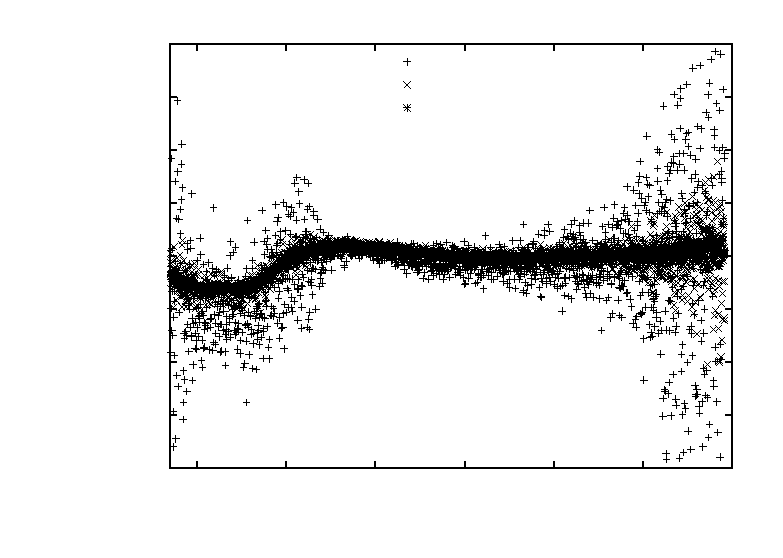
\includegraphics{TPE3}}%
    \gplfronttext
  \end{picture}%
\endgroup

\caption{Naměřené spektrum v pro různé množství měření a integrační doby spektra.}
\label{TPE3}
\end{figure}


\section{Modulační metoda}
Druhá aparatura, kterou používáme je na obrázku (\ref{Schema modul}). Sestává z monochromátoru, polarizátoru, Faradayovy nulovací cely, Faradayovy modulační cely, fázové destičky, vzorku v magnetickém poli, analyzátoru zkříženým s polarizátorem a fotonásobiče s detektorem. 
X %TODO Faradayovy cely
Opět můžeme vyjádřit Jonesův vektor světla na detektoru
\begin{eqnarray}
J=\begin{bmatrix}0&0\\0&1\end{bmatrix}
\begin{bmatrix}r_{ss}&r_{sp}\\r_{ps}& r_{pp}\end{bmatrix}
\begin{bmatrix}e^{i\frac{\delta}{2}}&0\\0&e^{-i\frac{\delta}{2}}\end{bmatrix}
\begin{bmatrix}\cos(\beta_0\sin\omega_mt) & -\sin(\beta_0\sin\omega_mt) \\ \sin(\beta_0\sin\omega_mt)&\cos(\beta_0\sin\omega_mt)\end{bmatrix}
\begin{bmatrix}\cos\eta&-\sin\eta\\\sin\eta&\cos\eta\end{bmatrix}
\begin{bmatrix}\sin\alpha\\\cos\alpha\end{bmatrix} \\
=\begin{bmatrix}0\\\cos\eta(r_{ps}e^{i\frac{\delta}{2}}\cos\tau+r_{pp}e^{-i\frac{\delta}{2}}\sin\tau)& -\sin\eta(r_{ps}e^{i\frac{\delta}{2}}\sin\tau-t_{pp}e^{-i\frac{\delta}{2}}\cos\tau)\end{bmatrix};\\ \tau = \beta_0\sin\omega_mt
\end{eqnarray}
Po další úpravách, které jsou podrobněji rozebrány například v \ref{Nyvlt} získáme vztah pro intenzitu
\begin{eqnarray}
I\approx\frac{1}{2}\left[|r_{ps}|^2+|r_{pp}|^2(\eta+\tau)+(r_{ps}r^*_{pp}e^{i\delta})^2+r^*_{ps}r_{pp}e^{-i\delta})(\eta+\tau)\right]
\end{eqnarray}
a oscilující komponenta při $\omega_m$ je
\begin{eqnarray}
I_{\omega_m}\approx|r_{pp}|^2\left[\eta+\mbox{Re}\left(\frac{r_{ps}}{r_{pp}}e^{i\delta}\right)\right]\tau
\end{eqnarray}
X %TODO Zmínit, že se využívá synchronní detekce - detekuje se pouze oscilující složka na frekvenci omega_m



\section{Zařízení}
Nová aparatrura obsahuje monochromátor TRIAX 550. Jedná se o mřížkový monochromátor s možností volby z různých mřížek. V našem případě máme na výběr 600, 900 a 1200 vrypů na mm. Parametry těchto mřížek jsou uvedeny v tabulce (\ref{TTriax}). Tento monochromátor lze ovládat za pomoci rozhraní GPIB. 
\begin{table}
$$
\begin{array}{|c|c|c|}
\hline
\mbox{grating} [g/mm]&  \mbox{Disperze} [nm/mm]&    \mbox{Spektrální rozsah} [nm] \\ \hline
600&    2.83&   0 - 3000 \\ \hline
900&    1.84&   0 - 2000 \\ \hline
1200&   1.34&   0 - 1500 \\ \hline
\end{array}
$$
\caption{Parametry mřížek monochromátoru}
\label{TTriax}
\end{table}

K Určení velikosti signálu na fotonásobiči používáme mulimetr Keithley 2001. V našem případě v měříme napětí na rozsahu 1 V při kterém má přesnost $\pm(0.0045\%+0.0008)$V. Možnost automatického rozsahu nepoužíváme, protože při přepnutí rozsahu dochází ke skokům napětí. Komunikace je opět zprostředkována rozhraním GPIB.

Jako zroj elektrického proudu pro magnet používáme zdroj stejnosměrbého proudu Kepco BOP. Standartně do magnetu pouštíme $\pm 2.5$A. Při této hodnotě je chyba proudu 0.1 mA. Při přepólování magnetu je nutné měnit proud postupně, jinak by mohlo dojít ke zkratu na zdroji. V našem případě používáme krok 0.05 A za 0.1 sekundy.

\section{Ovládací program Kerr2}
V rámci náplně této práce byl zcela přeprogramován ovládaví program kvůli novým komponentám.
%TODO zkrátit popis. + obrázek

\subsection{Nastavení experimentu}
Tento program má hned několik funkcí, které usnadňují nastavení experimetnu. První z nich umožňuje manuální nastavení proudu magnetem. Uživatel zadá požadovaný proud a program pomalu zvyšuje proud, dokud nedosáhne požadované hodnoty. Dálší mód nastaví monochromátor na požadovanou vlnovou délku a otevře štěrbiny. Toho se používá především pro nastavení prvků v experimentu.

\subsection{Měření spektra}
Program umožňuje proměření spektra ve zvoleném rozahu s libovolným krokem. Dále umožňuje nastavení tolerance chyby měření, čekací doby po změňe magnetizace, počet měření jednotlivé vlnové délky a kalibračních koeficientů pro výpočet energie signálu. Po zahájení měření program nejprve nastaví na monochromátoru měřenou vlnovou délku a zapne proud do magnetu. Proud je přidáván postupně kvůli možnému zkratu na zroji při rychlém přepólování. Každé spektrum se měří opakovaně dle zadání uživatele, přičemž v celém prlběhu měření je kontrolováno, zda nebyl překročen rozsah. V takovém případě se měření pozastaví, aby umožnilo manuální otočení polarizátoru a měření pokračuje znovu od poslední vlnové délky. Měření opět probíhá i pro opačnou magnetizaci, přičemž program umožňuje zadání počtu otáček potřebných pro navrácení do rozsahu po změně polarizace. Nakonec je pro danou vlnovou délku provedeno třetí měření s původní magnetizací a je zkontrolována odchylka od prvního měření. V případě příliš velké odchylky se měření opakuje. V průběhu celého měření je vykreslován graf, ze kterého je možné již při měření odhalit případné nespojitosti. Po skončení měření jsou data uložena do expterního souboru spolu se všemi parametry měření.

\subsection{Hysterzní smyčky}
Program dále umožňuje měření hysterzních smyček a to dvěma způsoby. První postupně proměří při zadané vlnové délce různé hodnoty proudu, přičemž postupuje od zadané hodnoty I do -I s krokem, který je rovněž zadán. Následně se stejným krokem vrátí do hodnoty I. V průběhu měření je opět kreslen graf.

Druhá metoda nese anglický název four loop. Spočívá v postupném proměření hodnot vzdálených o $\Delta$I od hodnoty proudu I resp -I, přičemž tato vzálenost roste se zadaným krokem. Prlběh proudu je znázorněn na obrázku (\ref{4-loop}). Podstatné je, že vždy dojde do hodnoty I resp. -I.
